\section{Merging in two-photon events}
\label{sec:merging}

The single-photon study isolates fragmentation, but a useful reconstruction
must also keep neighbouring showers separate. Increasing the nearestHigher distance
can recover a displaced shower while allowing links to another particle.
I therefore extended the displaced-gun studies to two photons and examined both
the reconstructed objects and the nearest-higher-density links that form them.
All results in this section use the default \cluethreed{} configuration.

\subsection{Controlled shower separation}

Two complementary generators control the separation of the photons. In the
distance scan, the photons have equal energies and parallel momenta, while
their production points are shifted symmetrically by $\pm s/2$ in a randomly
chosen transverse direction. The sampled separations are
$s=1,2,4,8,16$~cm. Both trajectories must satisfy the gun's geometrical
acceptance. This gives a controlled comparison as the displacement is varied,
without changing the opening angle at the same time. The distance study uses
50\,000 generated events.

In the opening-angle scan, the two photons instead share a production point
and their momenta are rotated symmetrically around a central direction. The
angles are $\Delta\theta=0.001,0.004,0.016,0.064,0.256$~rad. Their physical
separation then grows along the shower depth. The two scans consequently test
different geometries: parallel, transversely separated showers and showers
that diverge from a common point.

\begin{figure*}[!tp]
  \centering
  \begin{subfigure}{0.88\textwidth}
    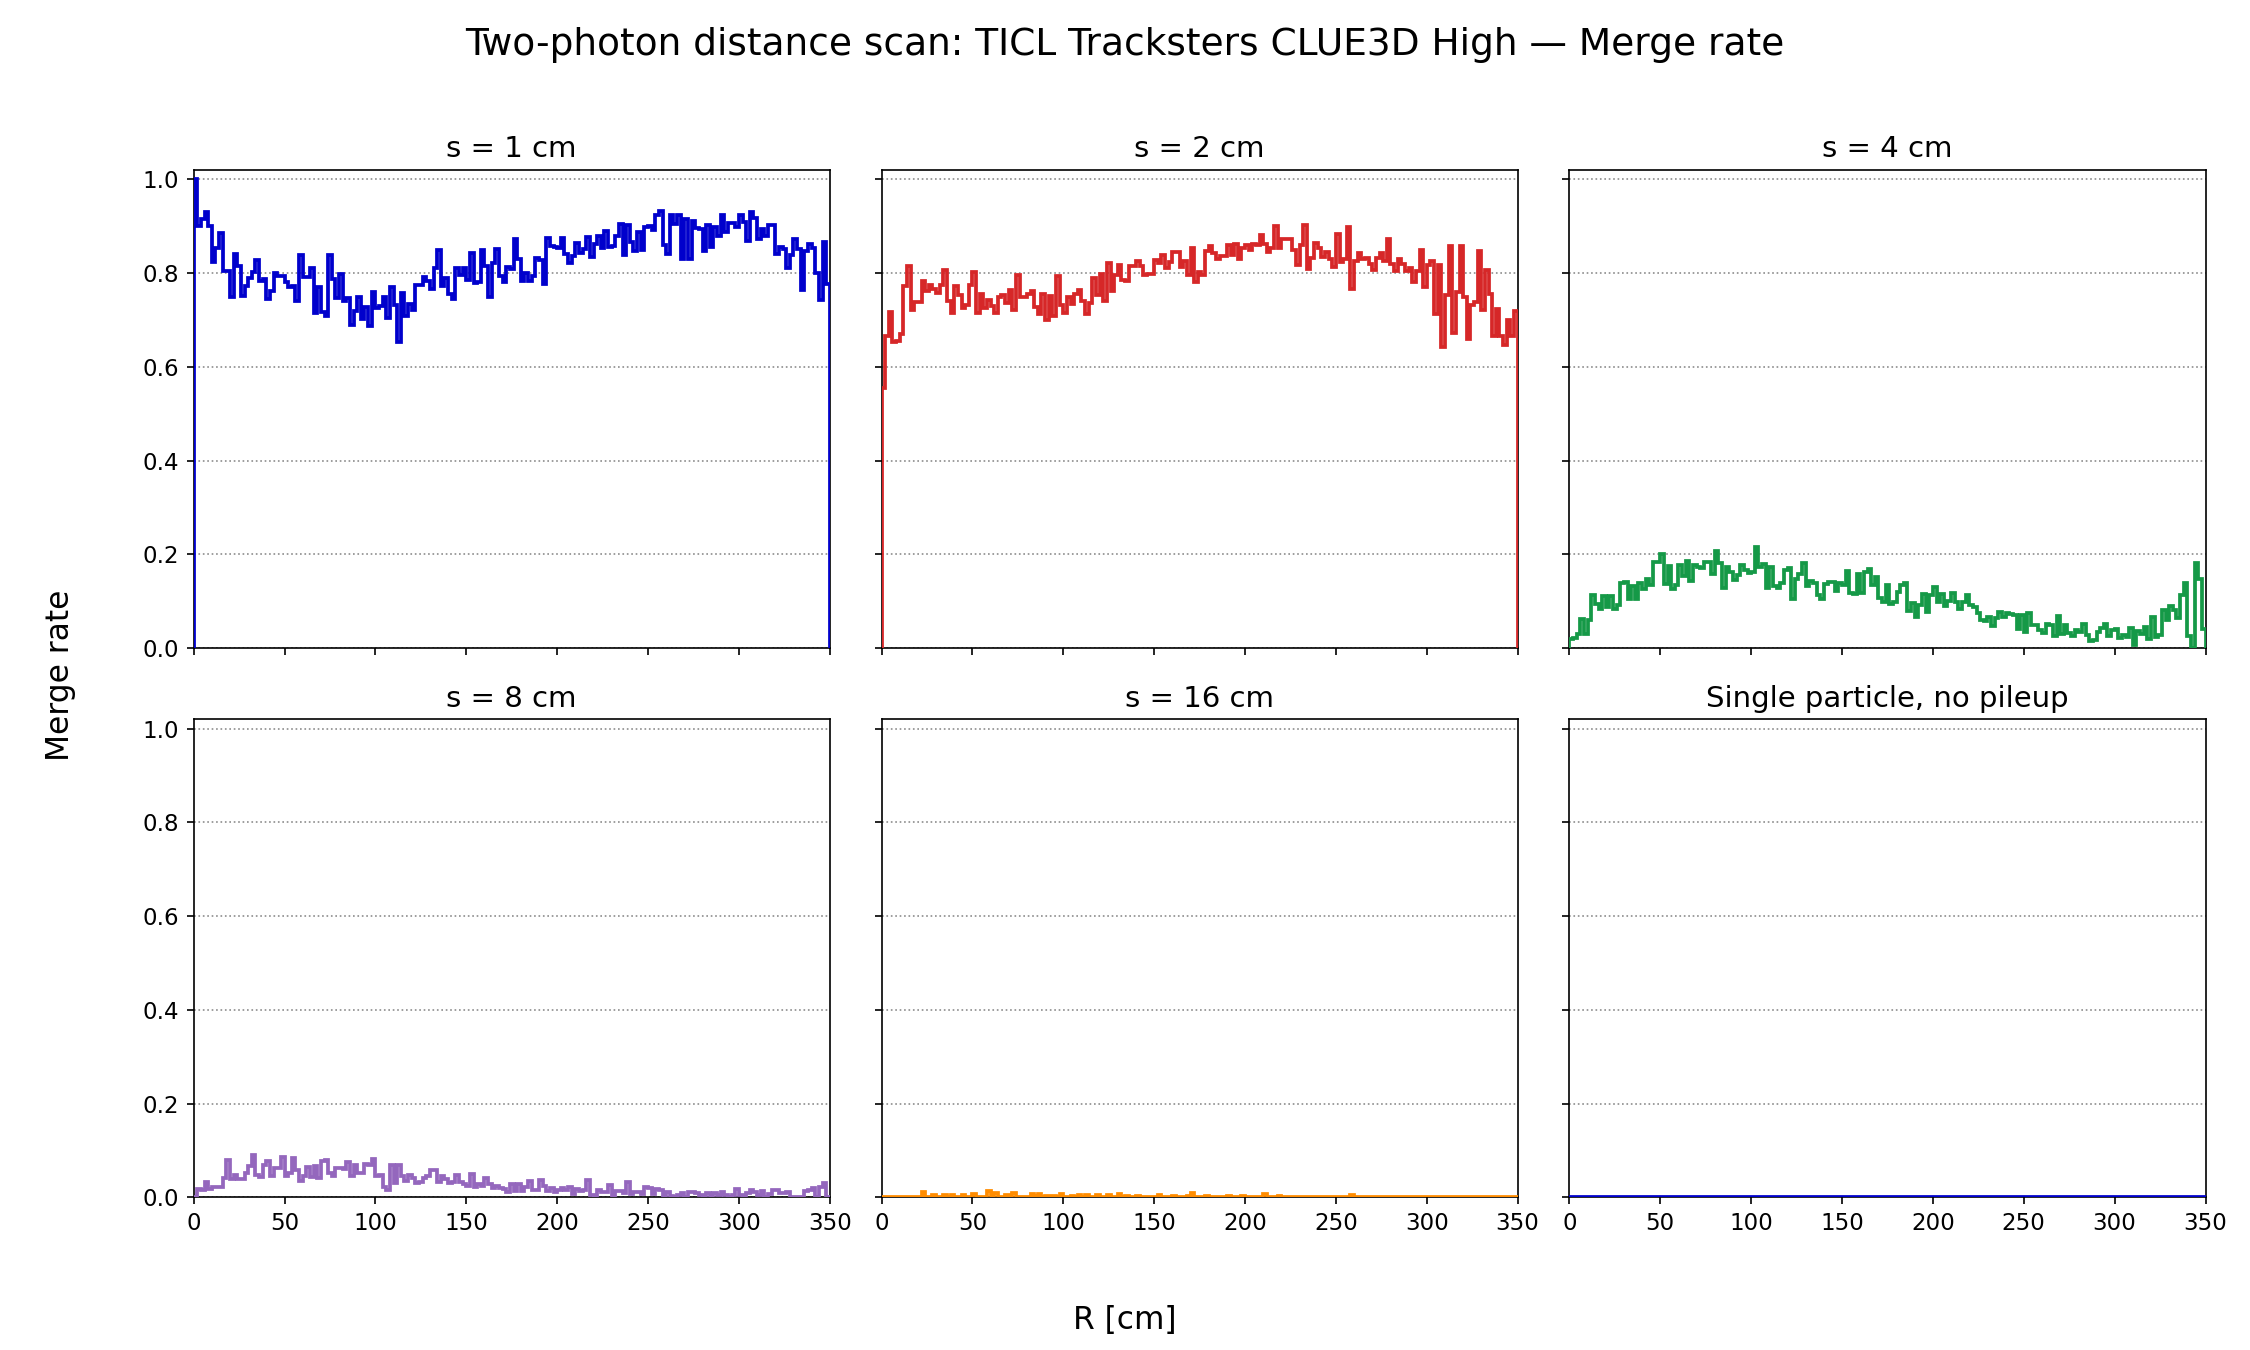
\includegraphics[width=\linewidth]{figures/merge_rate_distance.png}
    \caption{Reconstructed-object merge rate.}
    \label{fig:mergeratedistance}
  \end{subfigure}
  \par\medskip
  \begin{subfigure}{0.88\textwidth}
    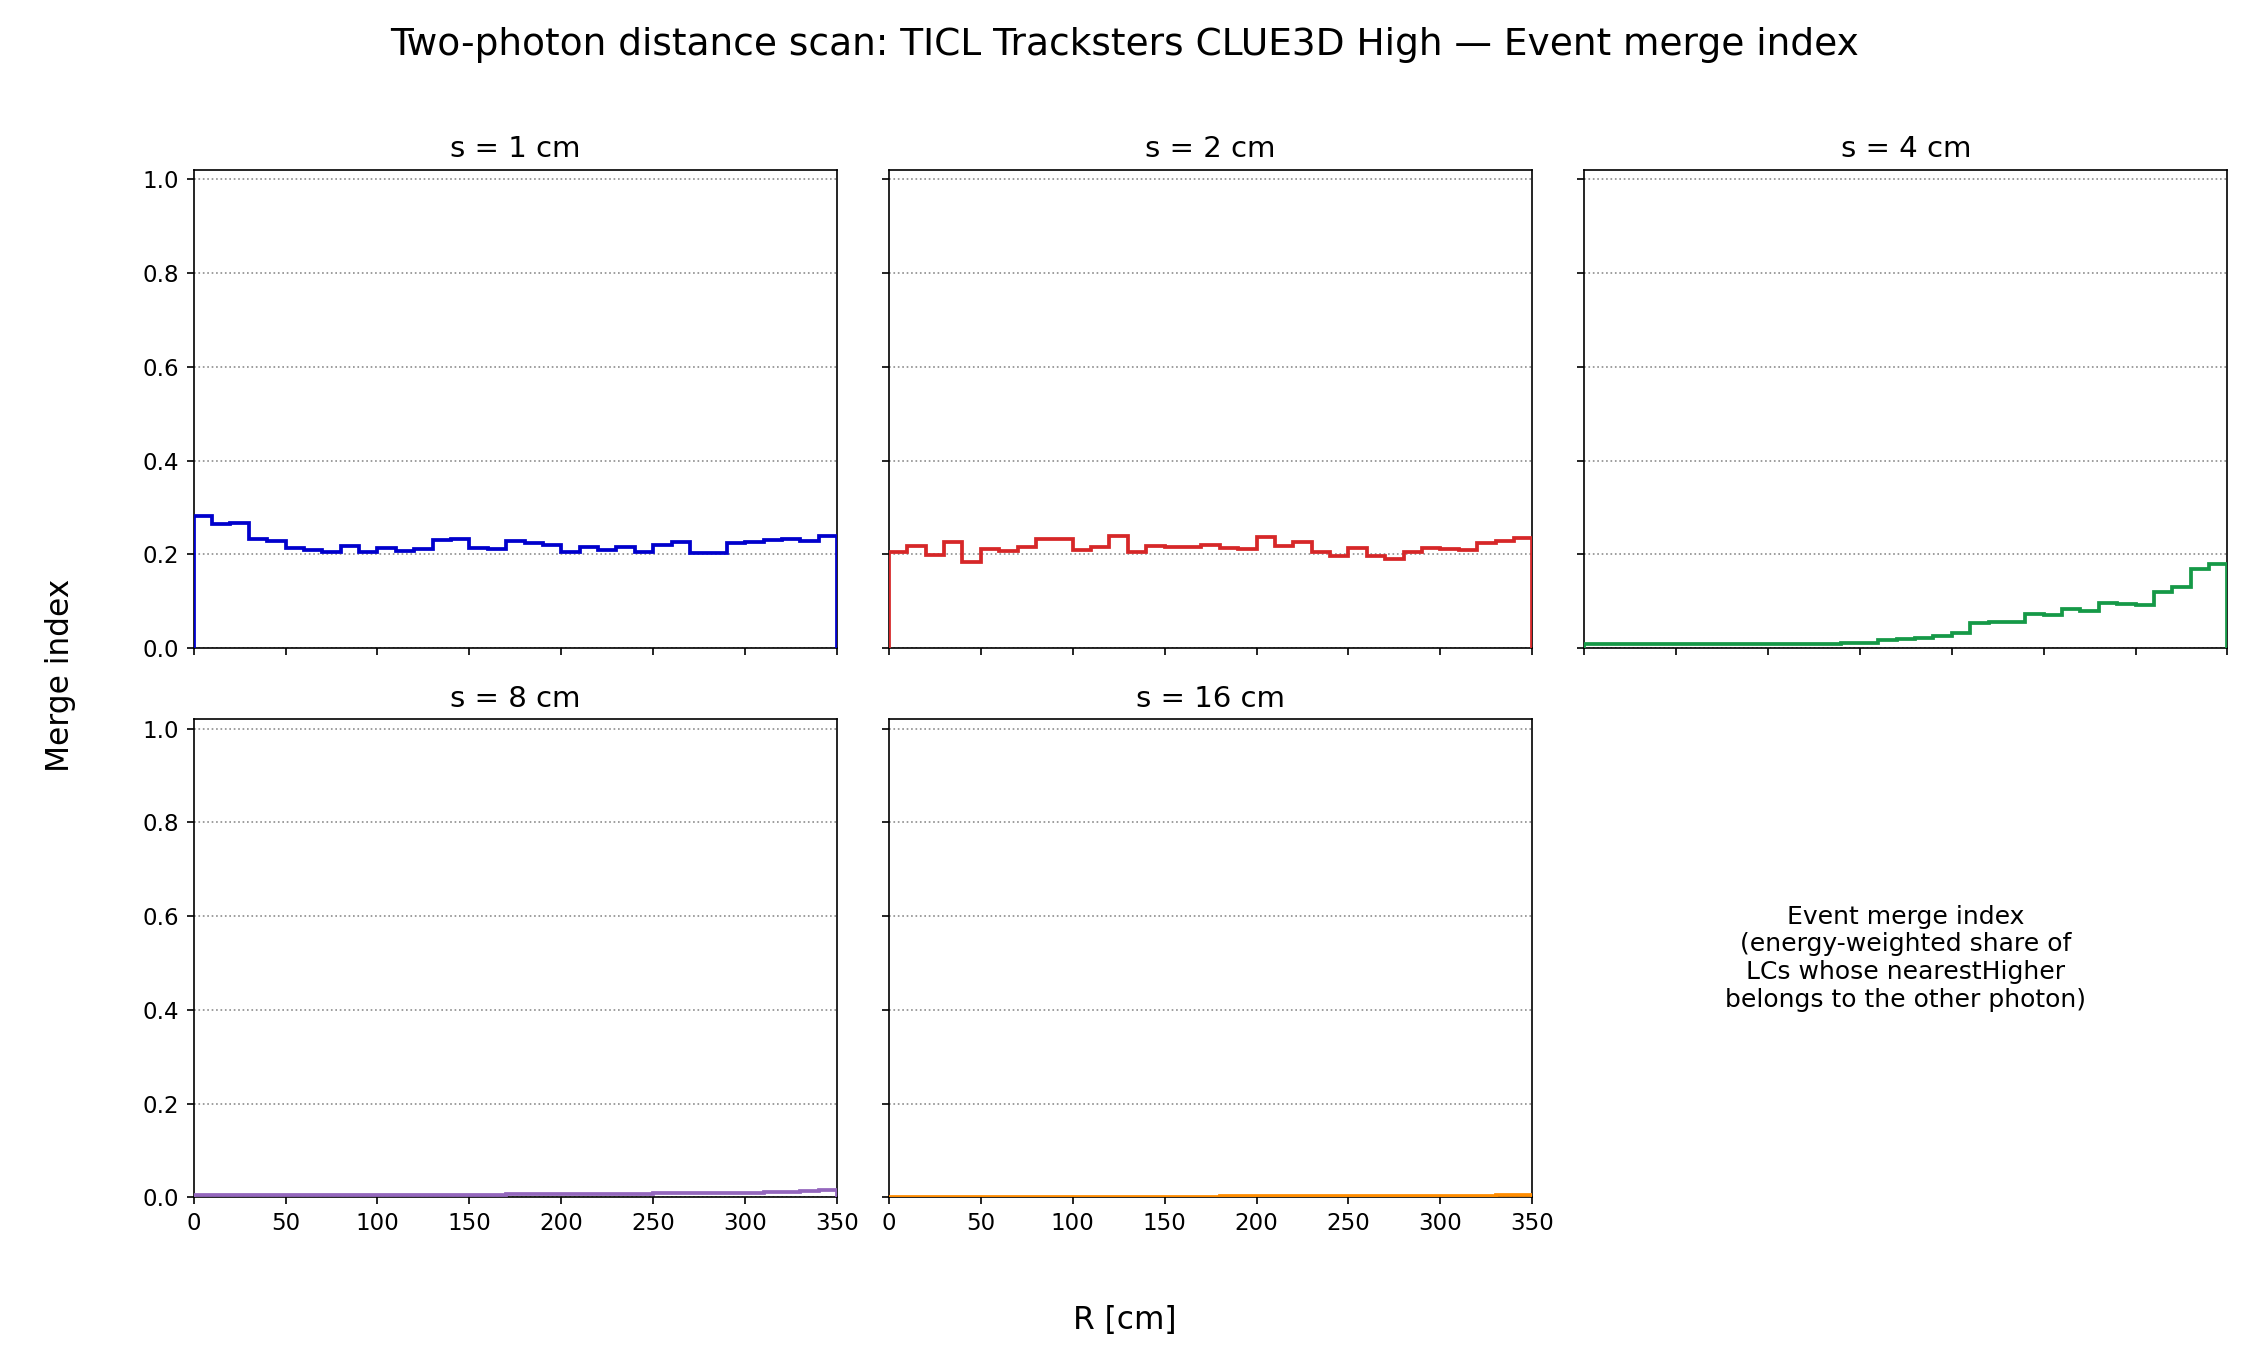
\includegraphics[width=\linewidth]{figures/merge_index_distance.png}
    \caption{Energy-weighted cross-shower link index.}
    \label{fig:mergeindexdistance}
  \end{subfigure}
  \caption{Two-photon distance scan with default \cluethreed{}. Each panel
  separates the five production-point distances. The object-based rate uses
  reconstructed $\R$, whereas the link index is binned using the truth
  displacement of the shower owning the follower LC. In particular, the
  $s=4$~cm index increases at large displacement even as the object-based merge
  rate falls.}
  \label{fig:mergingdistance}
\end{figure*}

For $s=4$~cm, the reconstructed-object merge rate initially appears
encouraging at large $\R$: after rising at intermediate displacement, it falls again
(Fig.~\ref{fig:mergeratedistance}). However, this is the same region in which
single showers fragment strongly. Splitting increases the number of
reconstructed objects in the denominator and can break an object that matched
two showers into smaller pieces that no longer pass both association cuts.
A decreasing merge rate therefore does not establish that the algorithm has
become better at separating the photons.

\subsection{A diagnostic based on the clustering links}

The object-based merge rate is distorted by fragmentation, so I introduced a
\emph{merge index} that measures cross-shower mixing directly from the
clustering links, without depending on how many Tracksters are produced. Every
follower LC $i$ records a nearest-higher neighbour $h(i)$; if $h(i)$ is owned by
a different truth shower than $i$, the algorithm has linked across the shower
boundary. The merge index is the energy-weighted fraction of follower energy in
such crossing links,
\begin{equation}
 I_{\mathrm{merge}}(B)=
 \frac{\sum_{i\in\mathcal{F}_B}E_i\,
 \mathbf{1}[o(h(i))\ne o(i),\ o(h(i))\text{ valid}]}
 {\sum_{i\in\mathcal{F}_B}E_i},
 \label{eq:mergeindex}
\end{equation}
where $o(\cdot)$ is the dominant truth-shower owner (the shower contributing the
largest truth energy fraction), $E_i$ the full LC energy, and $\mathcal{F}_B$
the truth-owned followers whose shower passes the truth selection in
displacement bin $B$ (seeds and outliers excluded). Energies are pooled across
the bin before the ratio is taken, so an index of $0.2$ means that $20\%$ of the
selected follower energy links into the wrong shower.

The index counts immediate links rather than the total energy ultimately
assigned to the wrong shower: one crossing link can redirect a whole chain of
followers, and seed and outlier decisions change which LCs enter the
denominator. These differences make it complementary to the object-based merge
rate.

Figure~\ref{fig:mergeindexdistance} resolves the apparent improvement. For
$s=4$~cm, the index rises from close to zero near the origin to about $0.18$
at large displacement. Cross-shower linking becomes more frequent even while
the reconstructed-object merge rate decreases. At $s=1$ and $2$~cm, substantial
mixing is already present, with an index of order $0.2$; the $8$ and $16$~cm
samples remain much cleaner. An index around $0.2$ should not be interpreted
as partial success at separating two almost overlapping showers: many links
can stay within their own dense core even when both cores ultimately feed the
same reconstructed object.

\subsection{Connection to the projective geometry}

\begin{figure*}[!tp]
  \centering
  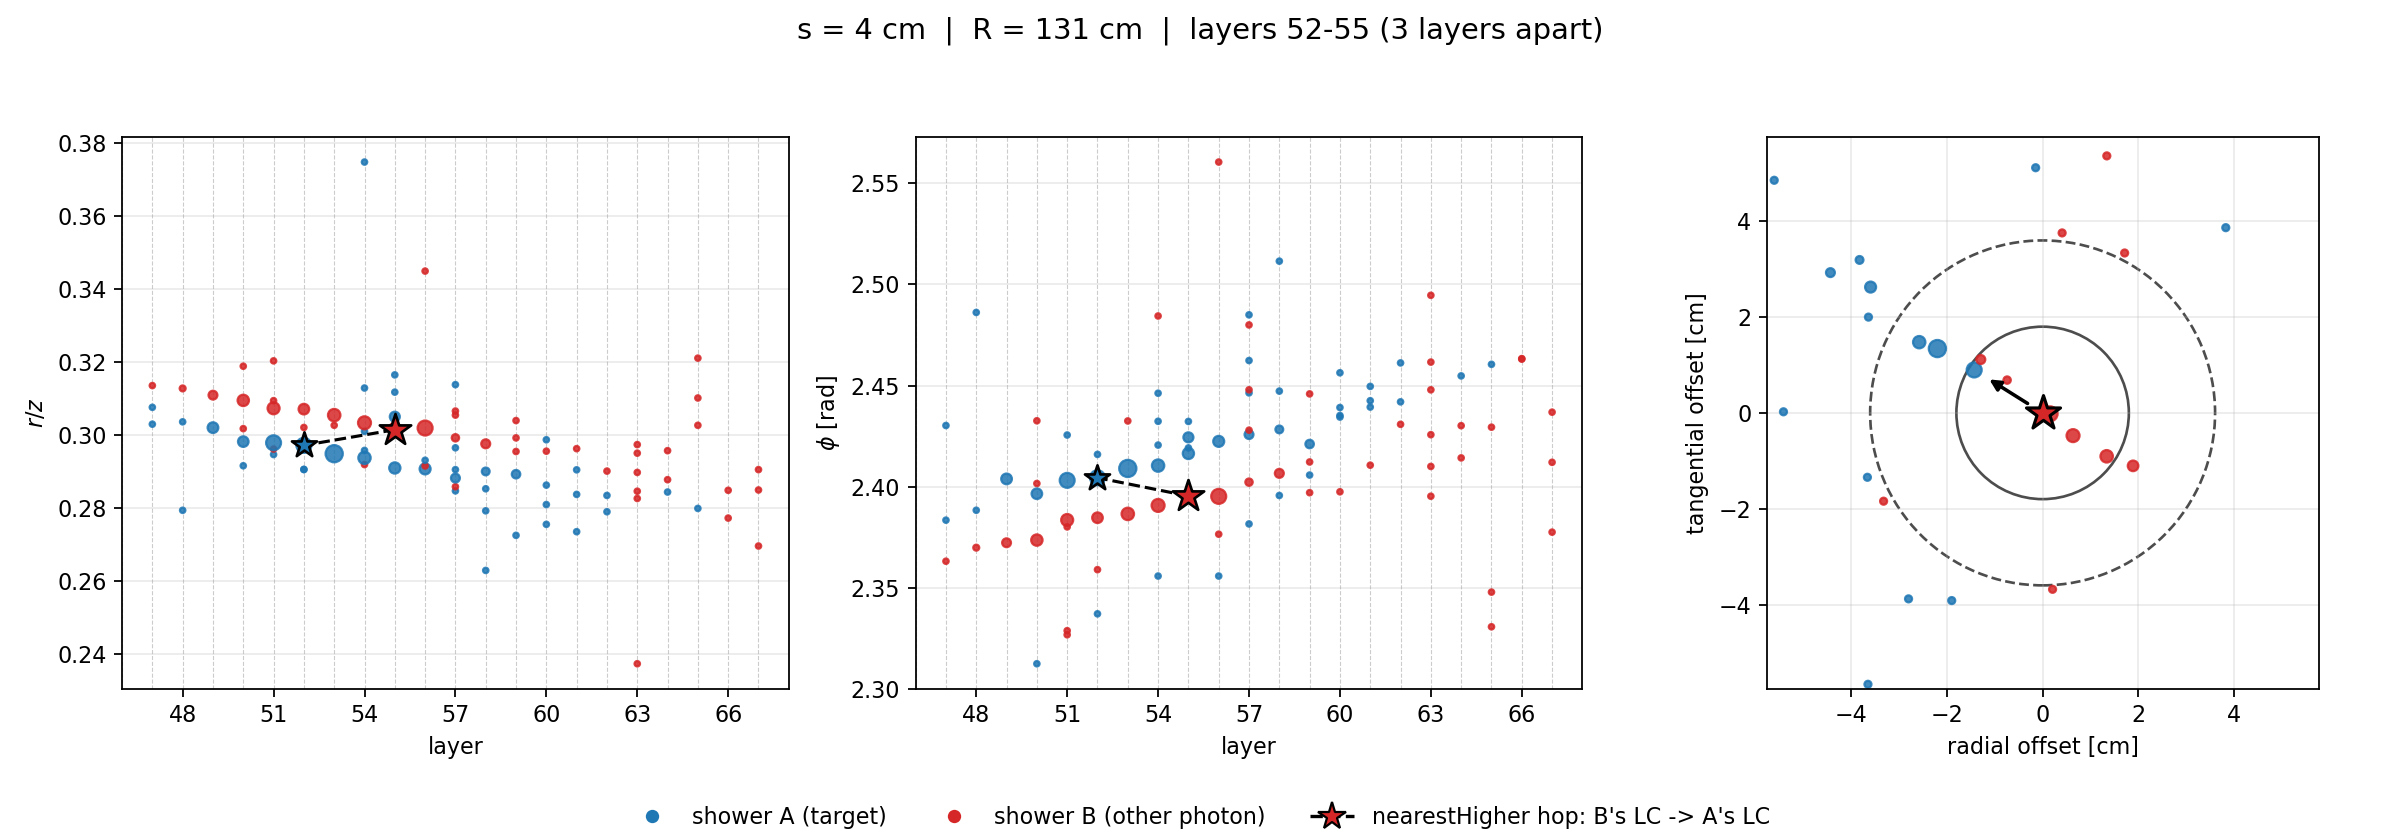
\includegraphics[width=\textwidth]{figures/merge_mechanism.png}
  \caption{An actual cross-shower nearest-higher link for photons separated
  by $s=4$~cm at $\R\simeq131$~cm. Blue and red identify the two truth
  showers. The highlighted LCs occupy layers 52 and 55, but have similar
  projective coordinates. The right panel shows neighbouring LCs projected
  onto the red LC's layer; the arrow follows its recorded link to shower
  $A$. The solid and dashed circles mark the 1.8~cm critical transverse
  distance and 3.6~cm outlier distance.}
  \label{fig:mergemechanism}
\end{figure*}

Figure~\ref{fig:mergemechanism} shows an individual cross-shower link, in an
event with $s=4$~cm and $\R\simeq131$~cm. The highlighted red LC belongs to
shower $B$, but its recorded nearest-higher neighbour is the blue LC from
shower $A$, three layers away. The first two panels show why this link is
geometrically possible: the two LCs have similar $r/|z|$ and $\phi$ despite
belonging to different showers, so that in the third panel the blue neighbour
lies inside the 1.8~cm circle once projected onto the red LC's layer. The
algorithm therefore sees a reachable higher-density neighbour across the truth
boundary, tying the cross-shower links to the observed merged objects.

The origin projection discussed in Section~\ref{sec:singlephoton} can also
explain how links cross between the showers. Consider ideal parallel axes
$\mathbf{x}_A(z)=\mathbf{b}_A+z\mathbf{a}$ and
$\mathbf{x}_B(z)=\mathbf{b}_A+\mathbf{s}+z\mathbf{a}$, where
$\mathbf{b}_A$ is shower $A$'s transverse intercept at $z=0$ and
$\mathbf{s}$ is their transverse separation, with $|\mathbf{s}|=s$. Projecting a point on shower
$B$ at $z_j$ onto the layer of a point on shower $A$ at $z_i$ gives distance:
\begin{equation}
 \mathbf{x}_A(z_i)-\frac{z_i}{z_j}\mathbf{x}_B(z_j)
 =\mathbf{b}_A\frac{z_j-z_i}{z_j}-\frac{z_i}{z_j}\mathbf{s}.
 \label{eq:crossshowerprojection}
\end{equation}
The first term is the displacement-induced offset derived for one shower;
the second represents the true separation of the pair. For suitable layer
ordering and separation direction, these terms partly cancel. Points from
different showers can then appear close in the projected plane even while
points along one shower are pushed apart.

\subsection{Which layer gaps produce the merging?}

\begin{figure*}[!tp]
  \centering
  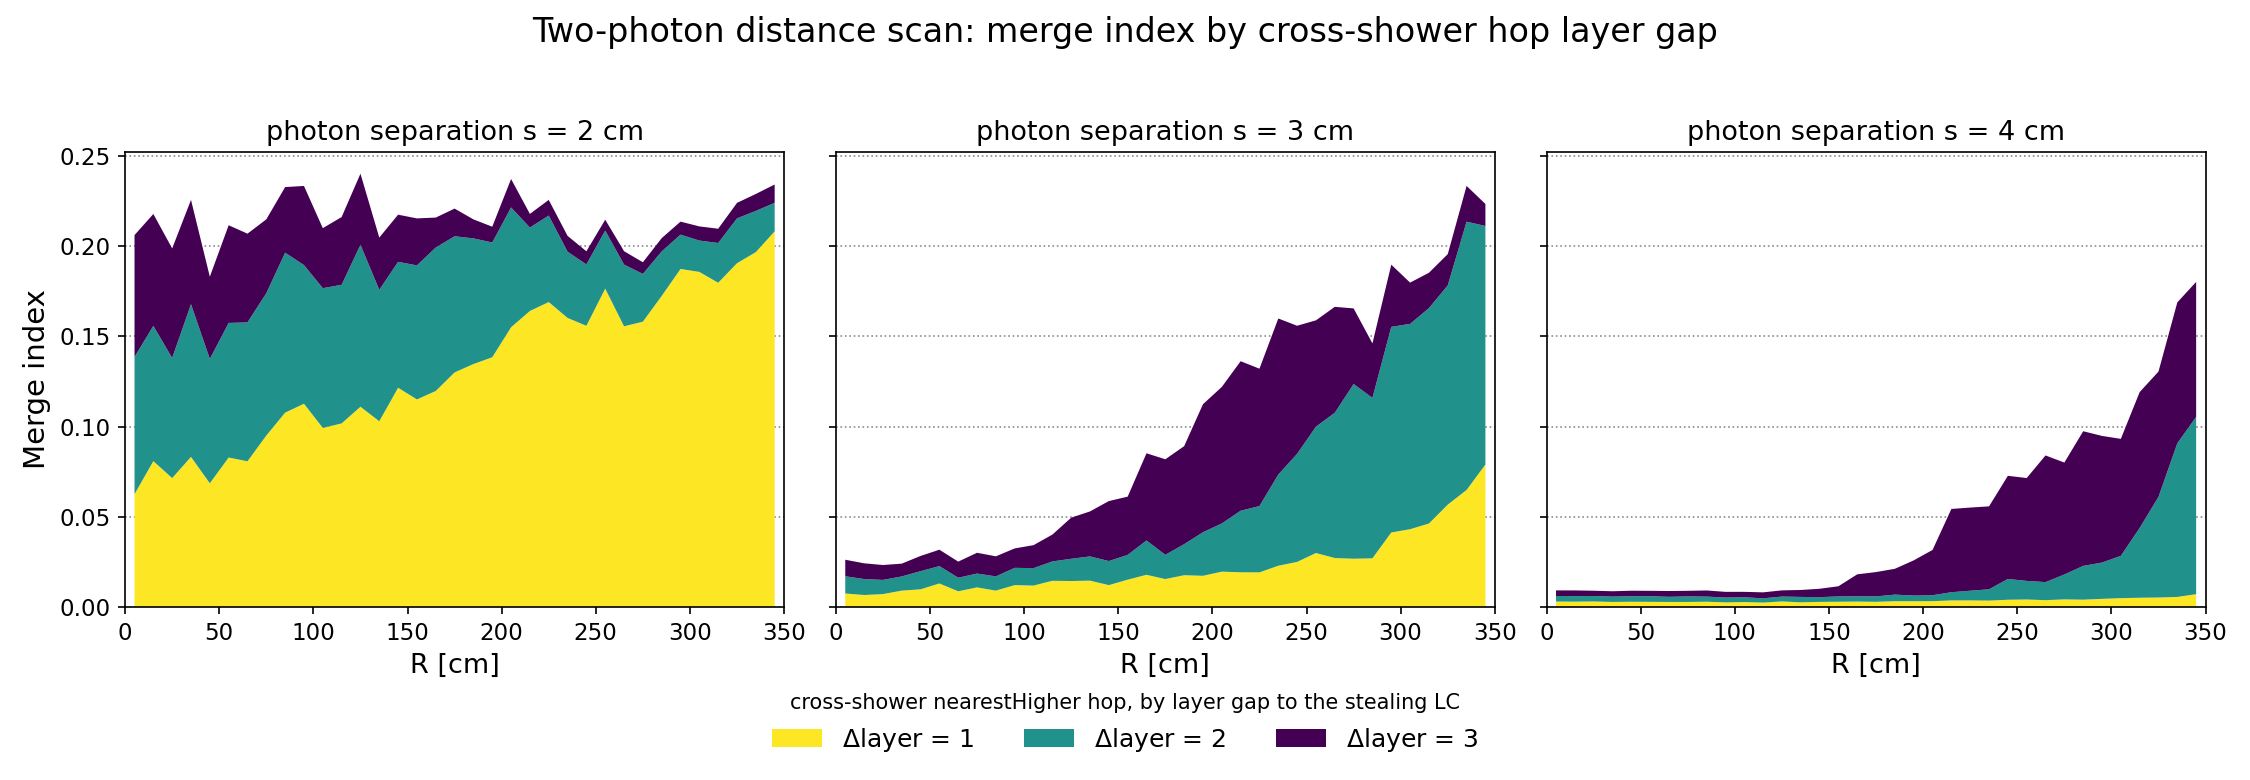
\includegraphics[width=\textwidth]{figures/merge_index_layergap.png}
  \caption{Merge index decomposed by the layer gap of cross-shower
  nearest-higher links for photon separations $s=2,3,4$~cm. Yellow, teal and
  purple correspond to one-, two- and three-layer gaps. All bands use the
  same follower-energy denominator, so their heights sum to the merge index.
  Larger separations favour larger gaps at the onset of mixing; increasing
  displacement makes smaller-gap contributions more important. The 3~cm
  panel comes from the finer separation scan.}
  \label{fig:mergegaps}
\end{figure*}

To see whether the three-layer link of Fig.~\ref{fig:mergemechanism} is
representative, I split the merge-index numerator by the layer gap
$\Delta\ell=|\ell_i-\ell_{h(i)}|$ between each follower and its cross-shower
neighbour, keeping the same denominator so the $\Delta\ell=1,2,3$ bands sum to
the merge index (Fig.~\ref{fig:mergegaps}, for $s=2,3,4$~cm).

The dominant gap shifts with separation. At $s=2$~cm, adjacent-layer links
carry most of the cross-shower energy and grow with $\R$. At $s=3$~cm the onset
is led by three-layer links, overtaken by two-layer links at larger $\R$. At
$s=4$~cm three-layer links dominate the onset and most of the growth, with
two-layer links rising only near the end of the scan. The event display of
Fig.~\ref{fig:mergemechanism} therefore shows the link type that drives the
onset for the $4$~cm pair, not an isolated coincidence.

This ordering follows from how the projection offset scales. Bridging the
separation $s$ requires offset, and since the offset grows with the
layer gap $\Delta z$, a wider gap reaches that offset at smaller $\R$. Wide-gap
links therefore start crossing first; as $\R$ increases, progressively
shorter-gap links reach the same offset and begin merging too. This is the
shift towards smaller gaps with displacement seen in the stacked bands, and it
explains not just that the merge index rises but which links carry the rise.

\subsection{Opening-angle scan}

\begin{figure*}[!tp]
  \centering
  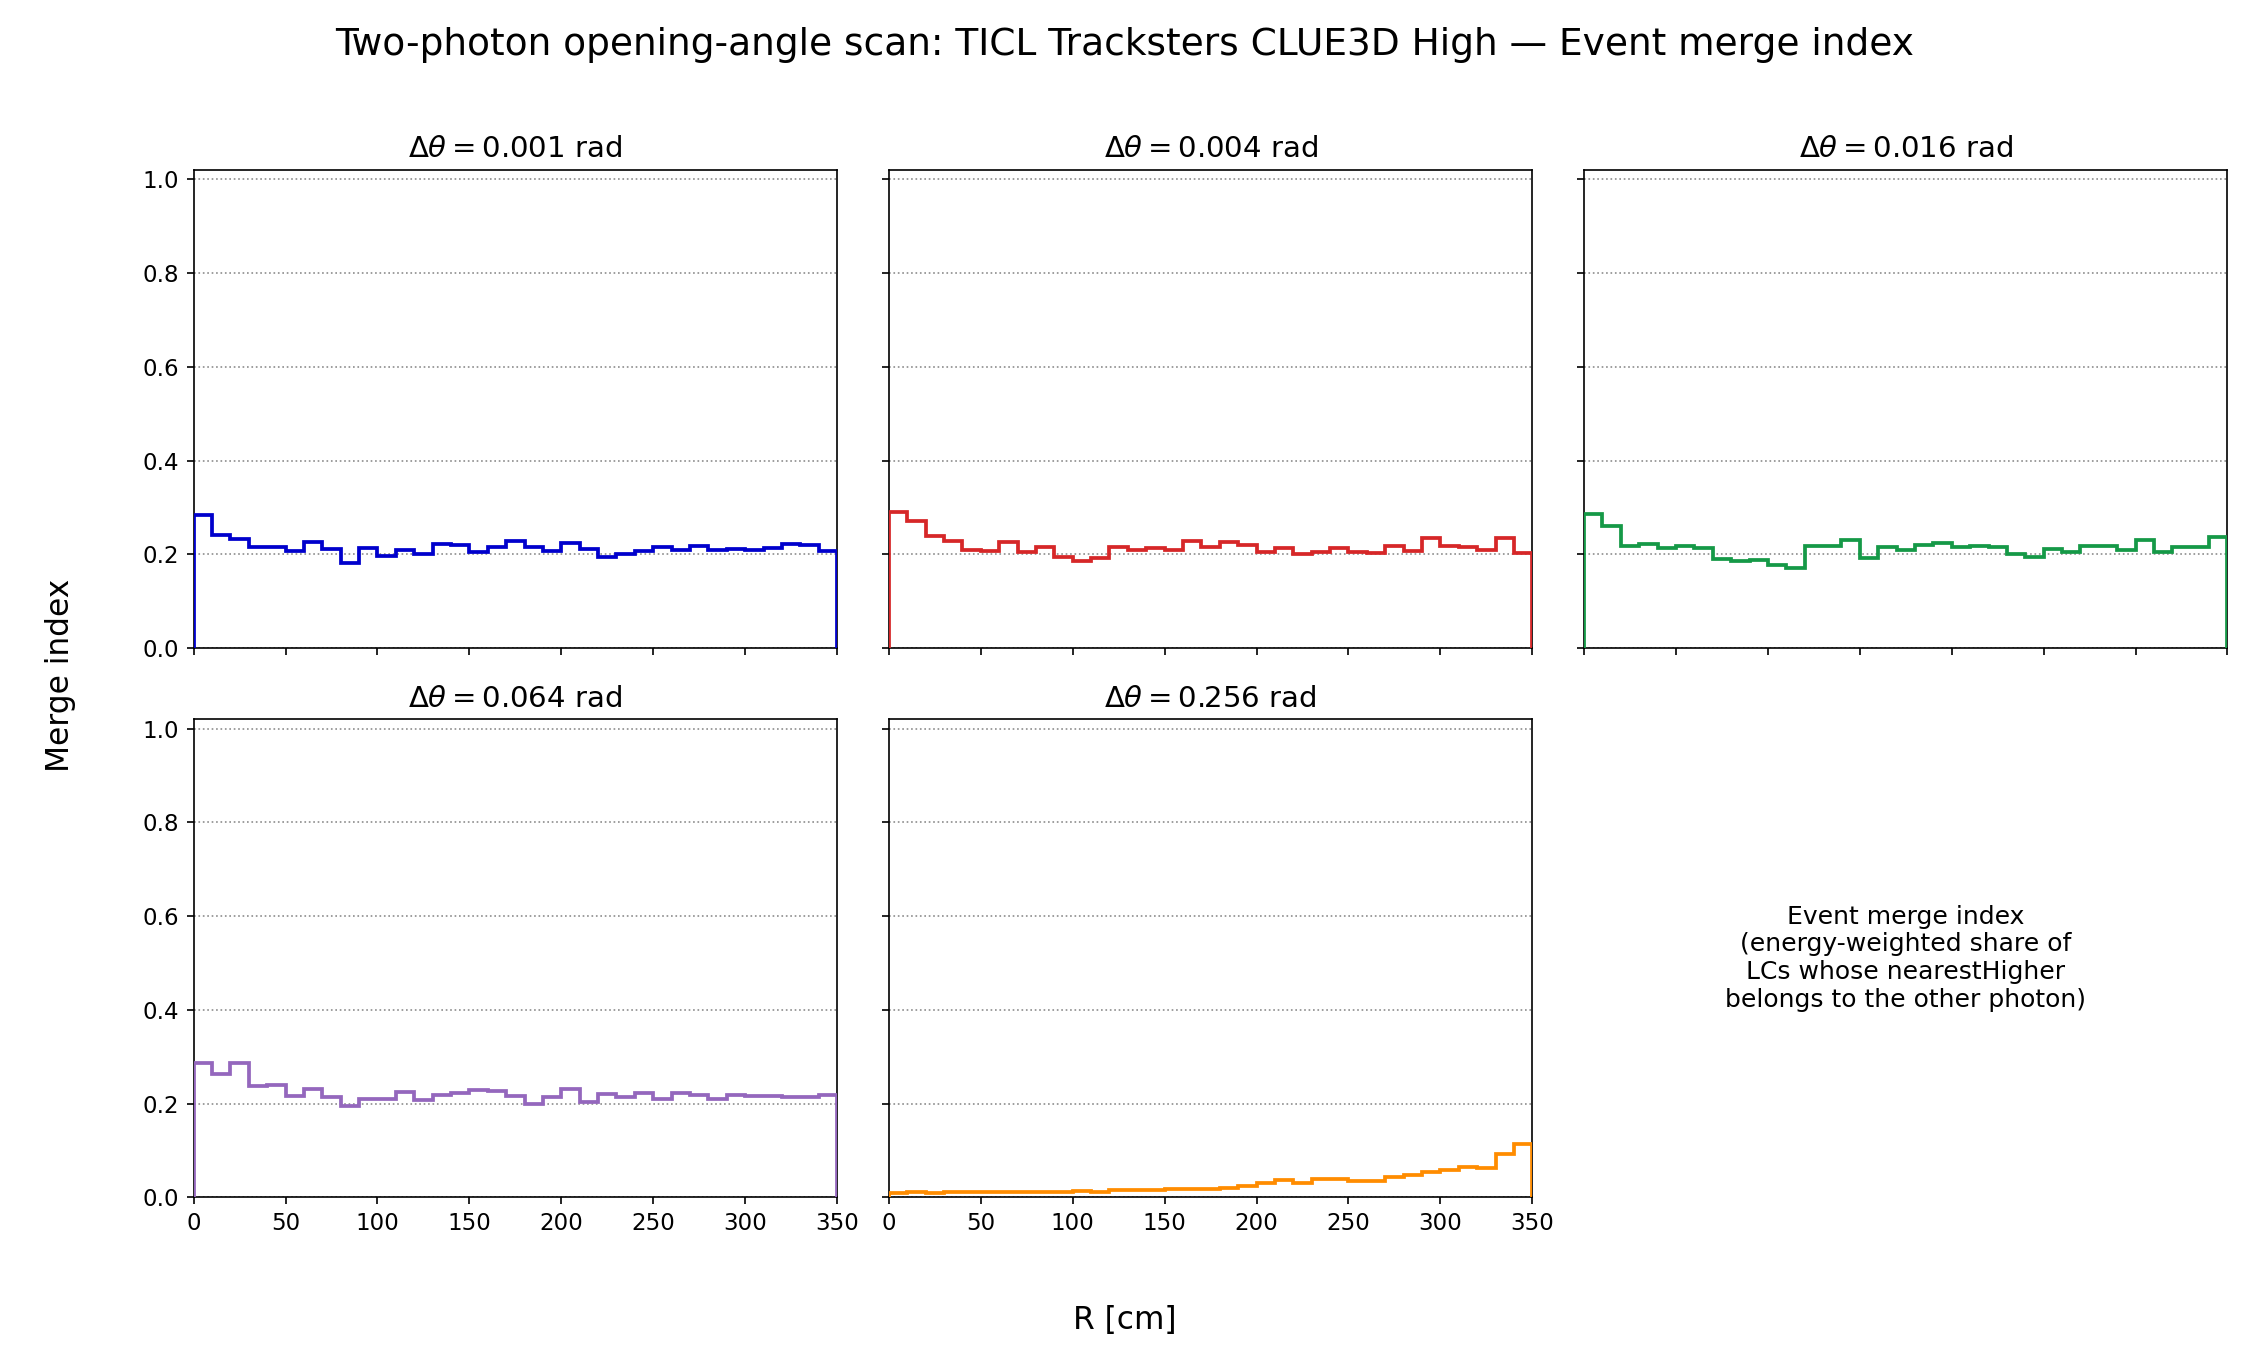
\includegraphics[width=0.86\textwidth]{figures/merge_index_theta.png}
  \caption{Merge index for the two-photon opening-angle scan. The index uses
  Eq.~\eqref{eq:mergeindex}, pooling follower energies within each bin. The largest opening angle provides the clearest
  increase in cross-shower linking with displacement.}
  \label{fig:mergeindextheta}
\end{figure*}

The opening-angle scan gives a complementary result
(Fig.~\ref{fig:mergeindextheta}). For the four smaller angles, the link index
is already substantial and remains near $0.2$ over most of the displacement
range. At the largest angle, $0.256$~rad, it starts near zero and increases
at large $\R$. A geometrically better-separated pair can therefore also lose
separation as displacement grows. Together, these scans show why tuning must
consider both shower completeness and cross-shower links: recovering energy
in larger Tracksters alone is not sufficient.

